%%
% Copyright (c) 2017 - 2023, Pascal Wagler;
% Copyright (c) 2014 - 2023, John MacFarlane
%
% All rights reserved.
%
% Redistribution and use in source and binary forms, with or without
% modification, are permitted provided that the following conditions
% are met:
%
% - Redistributions of source code must retain the above copyright
% notice, this list of conditions and the following disclaimer.
%
% - Redistributions in binary form must reproduce the above copyright
% notice, this list of conditions and the following disclaimer in the
% documentation and/or other materials provided with the distribution.
%
% - Neither the name of John MacFarlane nor the names of other
% contributors may be used to endorse or promote products derived
% from this software without specific prior written permission.
%
% THIS SOFTWARE IS PROVIDED BY THE COPYRIGHT HOLDERS AND CONTRIBUTORS
% "AS IS" AND ANY EXPRESS OR IMPLIED WARRANTIES, INCLUDING, BUT NOT
% LIMITED TO, THE IMPLIED WARRANTIES OF MERCHANTABILITY AND FITNESS
% FOR A PARTICULAR PURPOSE ARE DISCLAIMED. IN NO EVENT SHALL THE
% COPYRIGHT OWNER OR CONTRIBUTORS BE LIABLE FOR ANY DIRECT, INDIRECT,
% INCIDENTAL, SPECIAL, EXEMPLARY, OR CONSEQUENTIAL DAMAGES (INCLUDING,
% BUT NOT LIMITED TO, PROCUREMENT OF SUBSTITUTE GOODS OR SERVICES;
% LOSS OF USE, DATA, OR PROFITS; OR BUSINESS INTERRUPTION) HOWEVER
% CAUSED AND ON ANY THEORY OF LIABILITY, WHETHER IN CONTRACT, STRICT
% LIABILITY, OR TORT (INCLUDING NEGLIGENCE OR OTHERWISE) ARISING IN
% ANY WAY OUT OF THE USE OF THIS SOFTWARE, EVEN IF ADVISED OF THE
% POSSIBILITY OF SUCH DAMAGE.
%%

%%
% This is the Eisvogel pandoc LaTeX template.
%
% For usage information and examples visit the official GitHub page:
% https://github.com/Wandmalfarbe/pandoc-latex-template
%%

% Options for packages loaded elsewhere
\PassOptionsToPackage{unicode}{hyperref}
\PassOptionsToPackage{hyphens}{url}
\PassOptionsToPackage{dvipsnames,svgnames,x11names,table}{xcolor}
%
\documentclass[
  paper=a4,
  ,captions=tableheading
]{scrbook}
\usepackage{amsmath,amssymb}
% Use setspace anyway because we change the default line spacing.
% The spacing is changed early to affect the titlepage and the TOC.
\usepackage{setspace}
\setstretch{1.2}
\usepackage{iftex}
\ifPDFTeX
  \usepackage[T1]{fontenc}
  \usepackage[utf8]{inputenc}
  \usepackage{textcomp} % provide euro and other symbols
\else % if luatex or xetex
  \usepackage{unicode-math} % this also loads fontspec
  \defaultfontfeatures{Scale=MatchLowercase}
  \defaultfontfeatures[\rmfamily]{Ligatures=TeX,Scale=1}
\fi
\usepackage{lmodern}
\ifPDFTeX\else
  % xetex/luatex font selection
\fi
% Use upquote if available, for straight quotes in verbatim environments
\IfFileExists{upquote.sty}{\usepackage{upquote}}{}
\IfFileExists{microtype.sty}{% use microtype if available
  \usepackage[]{microtype}
  \UseMicrotypeSet[protrusion]{basicmath} % disable protrusion for tt fonts
}{}
\makeatletter
\@ifundefined{KOMAClassName}{% if non-KOMA class
  \IfFileExists{parskip.sty}{%
    \usepackage{parskip}
  }{% else
    \setlength{\parindent}{0pt}
    \setlength{\parskip}{6pt plus 2pt minus 1pt}}
}{% if KOMA class
  \KOMAoptions{parskip=half}}
\makeatother
\usepackage{xcolor}
\definecolor{default-linkcolor}{HTML}{A50000}
\definecolor{default-filecolor}{HTML}{A50000}
\definecolor{default-citecolor}{HTML}{4077C0}
\definecolor{default-urlcolor}{HTML}{4077C0}
% load footmisc in order to customize footnotes (footmisc has to be loaded before hyperref, cf. https://tex.stackexchange.com/a/169124/144087)
\usepackage[hang,flushmargin,bottom,multiple]{footmisc}
\setlength{\footnotemargin}{0.8em} % set space between footnote nr and text
\setlength{\footnotesep}{\baselineskip} % set space between multiple footnotes
\setlength{\skip\footins}{0.3cm} % set space between page content and footnote
\setlength{\footskip}{0.9cm} % set space between footnote and page bottom
\usepackage[margin=2.5cm,includehead=true,includefoot=true,centering,]{geometry}
\usepackage[export]{adjustbox}
\usepackage{graphicx}
\usepackage{listings}
\newcommand{\passthrough}[1]{#1}
\lstset{defaultdialect=[5.3]Lua}
\lstset{defaultdialect=[x86masm]Assembler}
% add backlinks to footnote references, cf. https://tex.stackexchange.com/questions/302266/make-footnote-clickable-both-ways
\usepackage{footnotebackref}
\usepackage{graphicx}
\makeatletter
\def\maxwidth{\ifdim\Gin@nat@width>\linewidth\linewidth\else\Gin@nat@width\fi}
\def\maxheight{\ifdim\Gin@nat@height>\textheight\textheight\else\Gin@nat@height\fi}
\makeatother
% Scale images if necessary, so that they will not overflow the page
% margins by default, and it is still possible to overwrite the defaults
% using explicit options in \includegraphics[width, height, ...]{}
\setkeys{Gin}{width=\maxwidth,height=\maxheight,keepaspectratio}
% Set default figure placement to htbp
\makeatletter
% Make use of float-package and set default placement for figures to H.
% The option H means 'PUT IT HERE' (as  opposed to the standard h option which means 'You may put it here if you like').
\usepackage{float}
\floatplacement{figure}{H}
\makeatother
\setlength{\emergencystretch}{3em} % prevent overfull lines
\providecommand{\tightlist}{%
  \setlength{\itemsep}{0pt}\setlength{\parskip}{0pt}}
\setcounter{secnumdepth}{-\maxdimen} % remove section numbering
\ifLuaTeX
\usepackage[bidi=basic]{babel}
\else
\usepackage[bidi=default]{babel}
\fi
\babelprovide[main,import]{british}
% get rid of language-specific shorthands (see #6817):
\let\LanguageShortHands\languageshorthands
\def\languageshorthands#1{}
\usepackage{float}
\let\origfigure\figure
\let\endorigfigure\endfigure
\renewenvironment{figure}[1][2] {
    \expandafter\origfigure\expandafter[H]
} {
    \endorigfigure
}
\ifLuaTeX
  \usepackage{selnolig}  % disable illegal ligatures
\fi
\IfFileExists{bookmark.sty}{\usepackage{bookmark}}{\usepackage{hyperref}}
\IfFileExists{xurl.sty}{\usepackage{xurl}}{} % add URL line breaks if available
\urlstyle{same}
\hypersetup{
  pdftitle={Poyo's guide to retro web development!},
  pdfauthor={Poyo!},
  pdflang={en-GB},
  hidelinks,
  breaklinks=true,
  pdfcreator={LaTeX via pandoc with the Eisvogel template}}
\title{Poyo's guide to retro web development!}
\author{Poyo!}
\date{v0.2}



%%
%% added
%%


%
% for the background color of the title page
%
\usepackage{pagecolor}
\usepackage{afterpage}
\usepackage[margin=2.5cm,includehead=true,includefoot=true,centering]{geometry}

%
% break urls
%
\PassOptionsToPackage{hyphens}{url}

%
% When using babel or polyglossia with biblatex, loading csquotes is recommended
% to ensure that quoted texts are typeset according to the rules of your main language.
%
\usepackage{csquotes}

%
% captions
%
\definecolor{caption-color}{HTML}{777777}
\usepackage[font={stretch=1.2}, textfont={color=caption-color}, position=top, skip=4mm, labelfont=bf, singlelinecheck=false, justification=raggedright]{caption}
\setcapindent{0em}

%
% blockquote
%
\definecolor{blockquote-border}{RGB}{221,221,221}
\definecolor{blockquote-text}{RGB}{119,119,119}
\usepackage{mdframed}
\newmdenv[rightline=false,bottomline=false,topline=false,linewidth=3pt,linecolor=blockquote-border,skipabove=\parskip]{customblockquote}
\renewenvironment{quote}{\begin{customblockquote}\list{}{\rightmargin=0em\leftmargin=0em}%
\item\relax\color{blockquote-text}\ignorespaces}{\unskip\unskip\endlist\end{customblockquote}}

%
% Source Sans Pro as the default font family
% Source Code Pro for monospace text
%
% 'default' option sets the default
% font family to Source Sans Pro, not \sfdefault.
%
\ifnum 0\ifxetex 1\fi\ifluatex 1\fi=0 % if pdftex
    \usepackage[default]{sourcesanspro}
  \usepackage{sourcecodepro}
  \else % if not pdftex
    \usepackage[default]{sourcesanspro}
  \usepackage{sourcecodepro}

  % XeLaTeX specific adjustments for straight quotes: https://tex.stackexchange.com/a/354887
  % This issue is already fixed (see https://github.com/silkeh/latex-sourcecodepro/pull/5) but the
  % fix is still unreleased.
  % TODO: Remove this workaround when the new version of sourcecodepro is released on CTAN.
  \ifxetex
    \makeatletter
    \defaultfontfeatures[\ttfamily]
      { Numbers   = \sourcecodepro@figurestyle,
        Scale     = \SourceCodePro@scale,
        Extension = .otf }
    \setmonofont
      [ UprightFont    = *-\sourcecodepro@regstyle,
        ItalicFont     = *-\sourcecodepro@regstyle It,
        BoldFont       = *-\sourcecodepro@boldstyle,
        BoldItalicFont = *-\sourcecodepro@boldstyle It ]
      {SourceCodePro}
    \makeatother
  \fi
  \fi

%
% heading color
%
\definecolor{heading-color}{RGB}{40,40,40}
\addtokomafont{section}{\color{heading-color}}
% When using the classes report, scrreprt, book,
% scrbook or memoir, uncomment the following line.
%\addtokomafont{chapter}{\color{heading-color}}

%
% variables for title, author and date
%
\usepackage{titling}
\title{Poyo's guide to retro web development!}
\author{Poyo!}
\date{v0.2}

%
% tables
%

%
% remove paragraph indentation
%
\setlength{\parindent}{0pt}
\setlength{\parskip}{6pt plus 2pt minus 1pt}
\setlength{\emergencystretch}{3em}  % prevent overfull lines

%
%
% Listings
%
%


%
% general listing colors
%
\definecolor{listing-background}{HTML}{F7F7F7}
\definecolor{listing-rule}{HTML}{B3B2B3}
\definecolor{listing-numbers}{HTML}{B3B2B3}
\definecolor{listing-text-color}{HTML}{000000}
\definecolor{listing-keyword}{HTML}{435489}
\definecolor{listing-keyword-2}{HTML}{1284CA} % additional keywords
\definecolor{listing-keyword-3}{HTML}{9137CB} % additional keywords
\definecolor{listing-identifier}{HTML}{435489}
\definecolor{listing-string}{HTML}{00999A}
\definecolor{listing-comment}{HTML}{8E8E8E}

\lstdefinestyle{eisvogel_listing_style}{
  language         = java,
  xleftmargin      = 0.6em,
  framexleftmargin = 0.4em,
  backgroundcolor  = \color{listing-background},
  basicstyle       = \color{listing-text-color}\linespread{1.0}%
                      \lst@ifdisplaystyle%
                      \small%
                      \fi\ttfamily{},
  breaklines       = true,
  frame            = single,
  framesep         = 0.19em,
  rulecolor        = \color{listing-rule},
  frameround       = ffff,
  tabsize          = 4,
  numberstyle      = \color{listing-numbers},
  aboveskip        = 1.0em,
  belowskip        = 0.1em,
  abovecaptionskip = 0em,
  belowcaptionskip = 1.0em,
  keywordstyle     = {\color{listing-keyword}\bfseries},
  keywordstyle     = {[2]\color{listing-keyword-2}\bfseries},
  keywordstyle     = {[3]\color{listing-keyword-3}\bfseries\itshape},
  sensitive        = true,
  identifierstyle  = \color{listing-identifier},
  commentstyle     = \color{listing-comment},
  stringstyle      = \color{listing-string},
  showstringspaces = false,
  escapeinside     = {/*@}{@*/}, % Allow LaTeX inside these special comments
  literate         =
  {á}{{\'a}}1 {é}{{\'e}}1 {í}{{\'i}}1 {ó}{{\'o}}1 {ú}{{\'u}}1
  {Á}{{\'A}}1 {É}{{\'E}}1 {Í}{{\'I}}1 {Ó}{{\'O}}1 {Ú}{{\'U}}1
  {à}{{\`a}}1 {è}{{\`e}}1 {ì}{{\`i}}1 {ò}{{\`o}}1 {ù}{{\`u}}1
  {À}{{\`A}}1 {È}{{\`E}}1 {Ì}{{\`I}}1 {Ò}{{\`O}}1 {Ù}{{\`U}}1
  {ä}{{\"a}}1 {ë}{{\"e}}1 {ï}{{\"i}}1 {ö}{{\"o}}1 {ü}{{\"u}}1
  {Ä}{{\"A}}1 {Ë}{{\"E}}1 {Ï}{{\"I}}1 {Ö}{{\"O}}1 {Ü}{{\"U}}1
  {â}{{\^a}}1 {ê}{{\^e}}1 {î}{{\^i}}1 {ô}{{\^o}}1 {û}{{\^u}}1
  {Â}{{\^A}}1 {Ê}{{\^E}}1 {Î}{{\^I}}1 {Ô}{{\^O}}1 {Û}{{\^U}}1
  {œ}{{\oe}}1 {Œ}{{\OE}}1 {æ}{{\ae}}1 {Æ}{{\AE}}1 {ß}{{\ss}}1
  {ç}{{\c c}}1 {Ç}{{\c C}}1 {ø}{{\o}}1 {å}{{\r a}}1 {Å}{{\r A}}1
  {€}{{\EUR}}1 {£}{{\pounds}}1 {«}{{\guillemotleft}}1
  {»}{{\guillemotright}}1 {ñ}{{\~n}}1 {Ñ}{{\~N}}1 {¿}{{?`}}1
  {…}{{\ldots}}1 {≥}{{>=}}1 {≤}{{<=}}1 {„}{{\glqq}}1 {“}{{\grqq}}1
  {”}{{''}}1
}
\lstset{style=eisvogel_listing_style}

%
% Java (Java SE 12, 2019-06-22)
%
\lstdefinelanguage{Java}{
  morekeywords={
    % normal keywords (without data types)
    abstract,assert,break,case,catch,class,continue,default,
    do,else,enum,exports,extends,final,finally,for,if,implements,
    import,instanceof,interface,module,native,new,package,private,
    protected,public,requires,return,static,strictfp,super,switch,
    synchronized,this,throw,throws,transient,try,volatile,while,
    % var is an identifier
    var
  },
  morekeywords={[2] % data types
    % primitive data types
    boolean,byte,char,double,float,int,long,short,
    % String
    String,
    % primitive wrapper types
    Boolean,Byte,Character,Double,Float,Integer,Long,Short
    % number types
    Number,AtomicInteger,AtomicLong,BigDecimal,BigInteger,DoubleAccumulator,DoubleAdder,LongAccumulator,LongAdder,Short,
    % other
    Object,Void,void
  },
  morekeywords={[3] % literals
    % reserved words for literal values
    null,true,false,
  },
  sensitive,
  morecomment  = [l]//,
  morecomment  = [s]{/*}{*/},
  morecomment  = [s]{/**}{*/},
  morestring   = [b]",
  morestring   = [b]',
}

\lstdefinelanguage{XML}{
  morestring      = [b]",
  moredelim       = [s][\bfseries\color{listing-keyword}]{<}{\ },
  moredelim       = [s][\bfseries\color{listing-keyword}]{</}{>},
  moredelim       = [l][\bfseries\color{listing-keyword}]{/>},
  moredelim       = [l][\bfseries\color{listing-keyword}]{>},
  morecomment     = [s]{<?}{?>},
  morecomment     = [s]{<!--}{-->},
  commentstyle    = \color{listing-comment},
  stringstyle     = \color{listing-string},
  identifierstyle = \color{listing-identifier}
}

%
% header and footer
%
\usepackage[headsepline,footsepline]{scrlayer-scrpage}

\newpairofpagestyles{eisvogel-header-footer}{
  \clearpairofpagestyles
  \ihead*{Poyo's guide to retro web development!}
  \chead*{}
  \ohead*{v0.2}
  \ifoot*{Poyo!}
  \cfoot*{}
  \ofoot*{\thepage}
  \addtokomafont{pageheadfoot}{\upshape}
}
\pagestyle{eisvogel-header-footer}

\deftripstyle{ChapterStyle}{}{}{}{}{\pagemark}{}
\renewcommand*{\chapterpagestyle}{ChapterStyle}


%%
%% end added
%%

\begin{document}

%%
%% begin titlepage
%%
\begin{titlepage}
\newgeometry{left=6cm}
\newcommand{\colorRule}[3][black]{\textcolor[HTML]{#1}{\rule{#2}{#3}}}
\begin{flushleft}
\noindent
\\[-1em]
\color[HTML]{5F5F5F}
\makebox[0pt][l]{\colorRule[435488]{1.3\textwidth}{8pt}}
\par
\noindent

{
  \setstretch{1.4}
  \vfill
  \noindent {\huge \textbf{\textsf{Poyo's guide to retro web development!}}}
    \vskip 2em
  \noindent {\Large \textsf{Poyo!}}
  \vfill
}

\noindent

\includegraphics[width=35mm, left]{images/still-poyo.png}

\textsf{v0.2}
\end{flushleft}
\end{titlepage}
\restoregeometry
\pagenumbering{arabic}

%%
%% end titlepage
%%

% \maketitle


{
\setcounter{tocdepth}{3}
\tableofcontents
\newpage
}
\hypertarget{prologue-by-woepdiecat}{%
\section{Prologue (By WoepdieCat)}\label{prologue-by-woepdiecat}}

I trust Poyo! to take this topic seriously and show you what websites
are really all about and the magic behind them

PD: He won't make it seriously, will he? Hahaha \newpage

\hypertarget{brief-introduction-to-the-book}{%
\section{Brief introduction to the
book}\label{brief-introduction-to-the-book}}

Howdy, internaut! If you're reading this book, I assume you're a
nostalgic peep who also wants to build a website reminiscent of the 90s.
However, you may have tried to build one, and have discovered that it's
challenging to create such beautiful pieces of art. That's why I'm here
to help you. :D

We will also dive on the trends of the 1990s-2000s, they are really
important to understand how can we replicate them. There were many
trends back in the 90s, such as having your visitors sign a guestbook,
visitor counters, and blinkies/buttons(More on that later), and believe
it or not, {Comic Sans} was all the rage worldwide. Yep O-O, Comic Sans.
What the fu-

Many of these trends originated because search engines were bad. Really
bad. So people linked their websites by entering on Webrings and by
sharing Buttons with their friends. Buttons are like souvenirs from
websites. These can be put on other's websites to show they liked the
website, or that they're friends of their corresponding webmaster. We'll
also talk about how to create a button yourself in this book.

In this book, I will teach you how to build your own website from
scratch, what were the trends in the 1990s-2000s and how can we
replicate the looks of such websites. Without further ado, let's get
started!

\begin{figure}
\centering
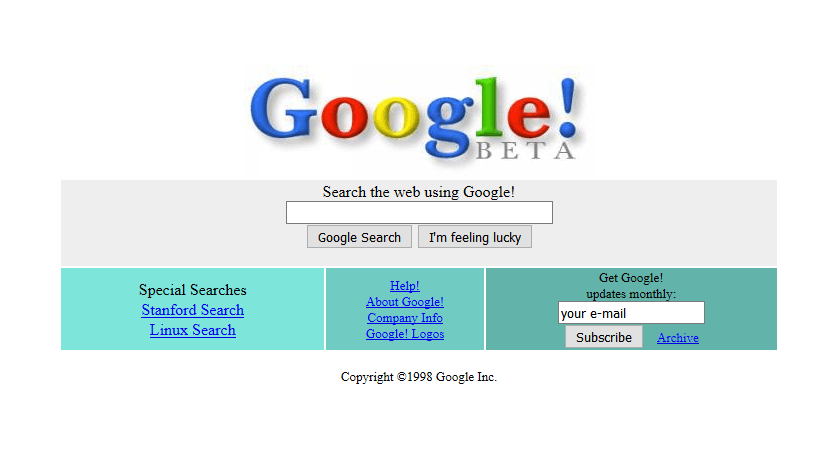
\includegraphics[width=1\textwidth,height=\textheight]{./tex2pdf.-45885137cafe410a/b955da96d4ab76fb1b756ca84c137b2b054fbd86.png}
\caption{This is how google looked in 1998. Image taken from
https://www.webdesignmuseum.org/exhibitions/web-design-in-the-90s}
\end{figure}

\hypertarget{chapter-1-vscode-and-web-development-tools}{%
\section{Chapter 1: VScode and Web Development
Tools}\label{chapter-1-vscode-and-web-development-tools}}

In this chapter, we will explore the powerful combination of Visual
Studio Code (VScode) and various web development tools that will be very
useful! \#\# 1.1.1 Getting Started with VScode

VScode is a popular code editor developed by Microsoft. It provides a
wide range of features and extensions that make it a favorite among many
web developers. To get started with
VScode\footnote{Official video-guide: https://www.youtube.com/watch?v=B-s71n0dHUk},
it's as simple as visiting their official
website\footnote{You can get VScode from https://code.visualstudio.com/.}
and downloading VScode. Afterwards, make sure to run the installation
wizard and you're now good to go!

\hypertarget{essential-extensions-for-web-development}{%
\subsection{1.1.2 Essential Extensions for Web
Development}\label{essential-extensions-for-web-development}}

VScode offers a huge collection of extensions that enhance the web
development experience. Here are some essential extensions to consider:

\begin{enumerate}
\def\labelenumi{\arabic{enumi}.}
\tightlist
\item
  \textbf{HTML CSS Support}: Provides autocompletion and syntax
  highlighting for HTML and CSS.
\item
  \textbf{Live Server}: Launches a local development server and
  automatically refreshes the browser whenever you make changes to your
  HTML, CSS, or JavaScript files. I personally love this extension
  because it makes web development so easy, that I can finish websites
  in a matter of minutes.
\item
  \textbf{Prettier}: Prettier automatically formats your code to ensure
  consistent styling and readability.
\item
  \textbf{Rainbow Indent}: It helps a lot with indenting and if you
  indent correctly, it will display a rainbow! :) Cool, isn't it?
\item
  \textbf{Live Share}: This extension allows you to share your local
  machine with your peers, so you can work collaboratively in a single
  dev environment! You can be editing one file while your peer edits
  another one. It's a must-have extension in my opinion.
\end{enumerate}

\hypertarget{collaboration-and-remote-development}{%
\subsection{1.1.3 Collaboration and Remote
Development}\label{collaboration-and-remote-development}}

VScode enables seamless collaboration and remote development. Here are
some features to consider:

\begin{enumerate}
\def\labelenumi{\arabic{enumi}.}
\tightlist
\item
  \textbf{Live Share}: With Live Share, you can share your development
  environment with others, allowing them to edit and debug code in
  real-time.
\item
  \textbf{GitHub Codespaces}: GitHub offers a service called Codespaces,
  which provides a cloud-based development environment with VSCode
  pre-installed. With Codespaces, you can access a Linux machine from
  anywhere in the world, making it convenient for remote development.
\end{enumerate}

\hypertarget{how-to-use-vscode}{%
\subsection{1.1.4 How to use VSCode?}\label{how-to-use-vscode}}

\begin{enumerate}
\def\labelenumi{\arabic{enumi}.}
\tightlist
\item
  \textbf{Opening a Project}: Once you have installed VSCode, open it
  and you will see the welcome screen. From there, you can either open
  an existing project or create a new one. To open an existing project,
  click on \enquote{Open Folder} and select the folder containing your
  project files.
\item
  \textbf{Editor Layout}: The VSCode interface consists of several
  components. The \emph{editor groups} are the editor, where you write
  your code. On the left side, you have the \emph{activity bar}, which
  provides access to different views like the file explorer, source
  control, extensions, and more. At the bottom, you have the
  \emph{status bar}, which displays information about the current file,
  a handy terminal and it also provides quick access to various
  settings.
\end{enumerate}

\begin{figure}
\centering
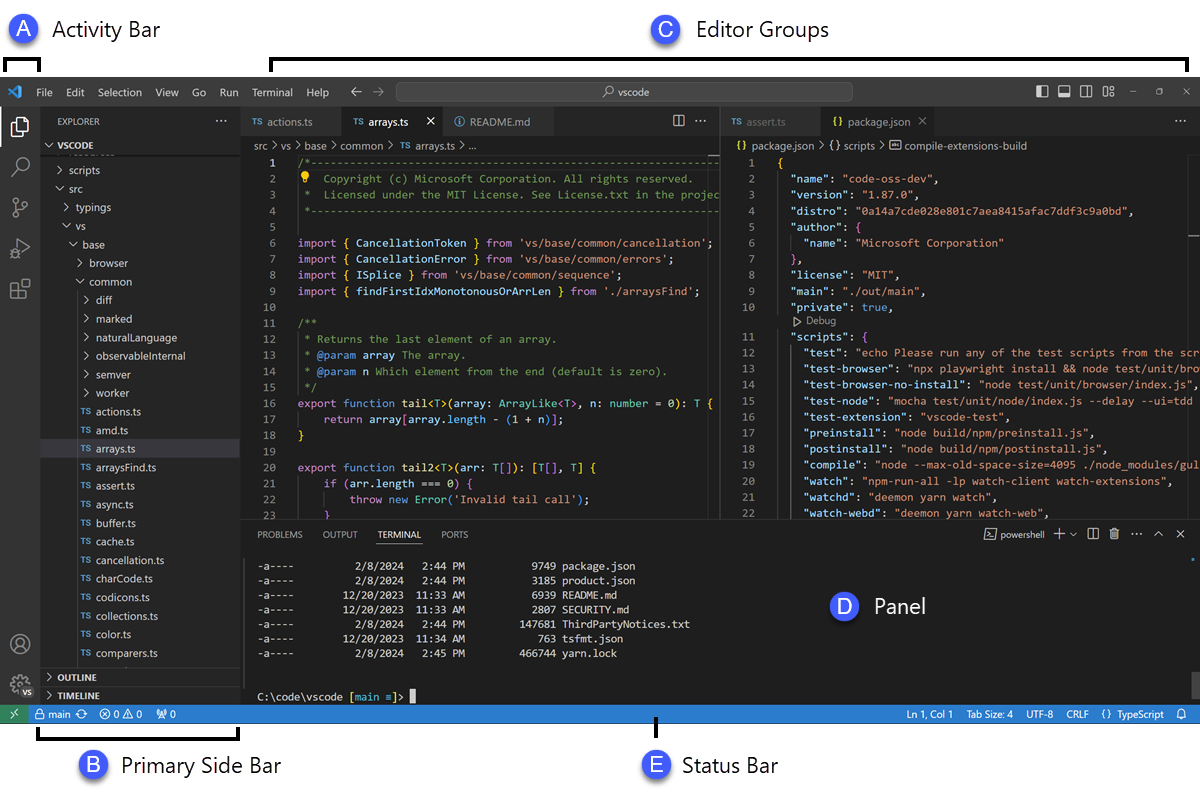
\includegraphics{./tex2pdf.-45885137cafe410a/adee506e3181b674ae69ce0359aac367163803c0.png}
\caption{VScode components}
\end{figure}

\begin{enumerate}
\def\labelenumi{\arabic{enumi}.}
\setcounter{enumi}{2}
\tightlist
\item
  \textbf{Terminal}: VScode has an integrated terminal to make coding
  easier. You can access it by opening the bottom bar. But be careful!
  It will be a live terminal running on your computer. I suggest doing
  all of your changes in a single folder and then, once you're finished,
  move all of the files inside to the location where you'll be running
  them.
\end{enumerate}

\hypertarget{git}{%
\subsection{1.2 Git}\label{git}}

\hypertarget{what-is-git}{%
\subsubsection{1.2.1 What is Git?}\label{what-is-git}}

\begin{figure}
\centering

\includegraphics[width=0.5\textwidth,height=\textheight]{./tex2pdf.-45885137cafe410a/b7be8868d46c63c4c032489b59e6c1abdb12b3cc.png}
\caption{Git's logo}
\end{figure}

Git is a widely used version control system. It's useful for having and
mantaining different versions of your code, and to store them in GitHub
for free. Git works by branches. Textually from Git's docs:

\begin{quote}
Branching means you diverge from the main line of development and
continue to do work without messing with that main line.
\end{quote}

What does that mean? In Git there is a \emph{main} branch, and then you
can create more branches to independently write code/features for your
project without messing up the \emph{main} branch, the current
\emph{working} code. Once you finish coding, you can pull the branch to
\emph{main} Thankfully, VScode offers excellent integration with Git,
which means we won't have to ever use any Git commands while using
VScode. Let's see how can we use it!

\begin{figure}
\centering
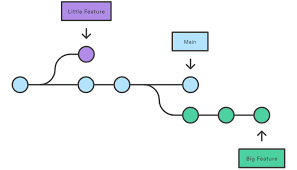
\includegraphics[width=0.5\textwidth,height=\textheight]{./tex2pdf.-45885137cafe410a/7f052acda8c69b8ef1156d1d65b0c0e1538337f6.png}
\caption{An example of a Git repository with its \emph{main}, \emph{big
feature} and \emph{little feature} branches.}
\end{figure}

\hypertarget{how-to-use-git}{%
\subsection{How to use git?}\label{how-to-use-git}}

Git is a command line tool. That means it can be accessed and used via
the terminal. The main Git
commands\footnote{Full list of commands available at https://confluence.atlassian.com/bitbucketserver/basic-git-commands-776639767.html}
are:

\begin{enumerate}
\def\labelenumi{\arabic{enumi}.}
\tightlist
\item
  To authenticate yourself:
\end{enumerate}

\begin{lstlisting}
git config --global user.name "<username>"
git config --global user.email <email>
\end{lstlisting}

\begin{enumerate}
\def\labelenumi{\arabic{enumi}.}
\setcounter{enumi}{1}
\tightlist
\item
  To start developing:

  \begin{itemize}
  \tightlist
  \item
    \passthrough{\lstinline!git init!} - Create a new repository
  \item
    \passthrough{\lstinline!git clone <repository url>!} - Download a
    copy of a repository to commit changes or just to use the code.
  \end{itemize}
\item
  To save your work

  \begin{itemize}
  \tightlist
  \item
    \passthrough{\lstinline!git add .!} - Add all the files changed to
    the commit.
  \item
    \passthrough{\lstinline!git commit -m "<Commit message>"!} - Commit
    changes to the head branch of your git repo(repository)
  \item
    \passthrough{\lstinline!git push!} - Send the changes and store them
    in the github repo
  \end{itemize}
\end{enumerate}

The github code to authenticate and retriev, we explored the powered how
to get started with VScode, essential extensions for web development,
debugging and testing capabilities, version control with Git, and
collaboration features. In the next chapter, we will learn about the
basics of building websites. See you there!

\end{document}